\documentclass[../main.tex]{subfiles}
%!TEX root = ./analysisThrusterArms.tex
\graphicspath {{../}}

\begin{document}
\subsection{Thruster Arms} \label{thrustArms}

\begin{figure}[H]
	\centering
	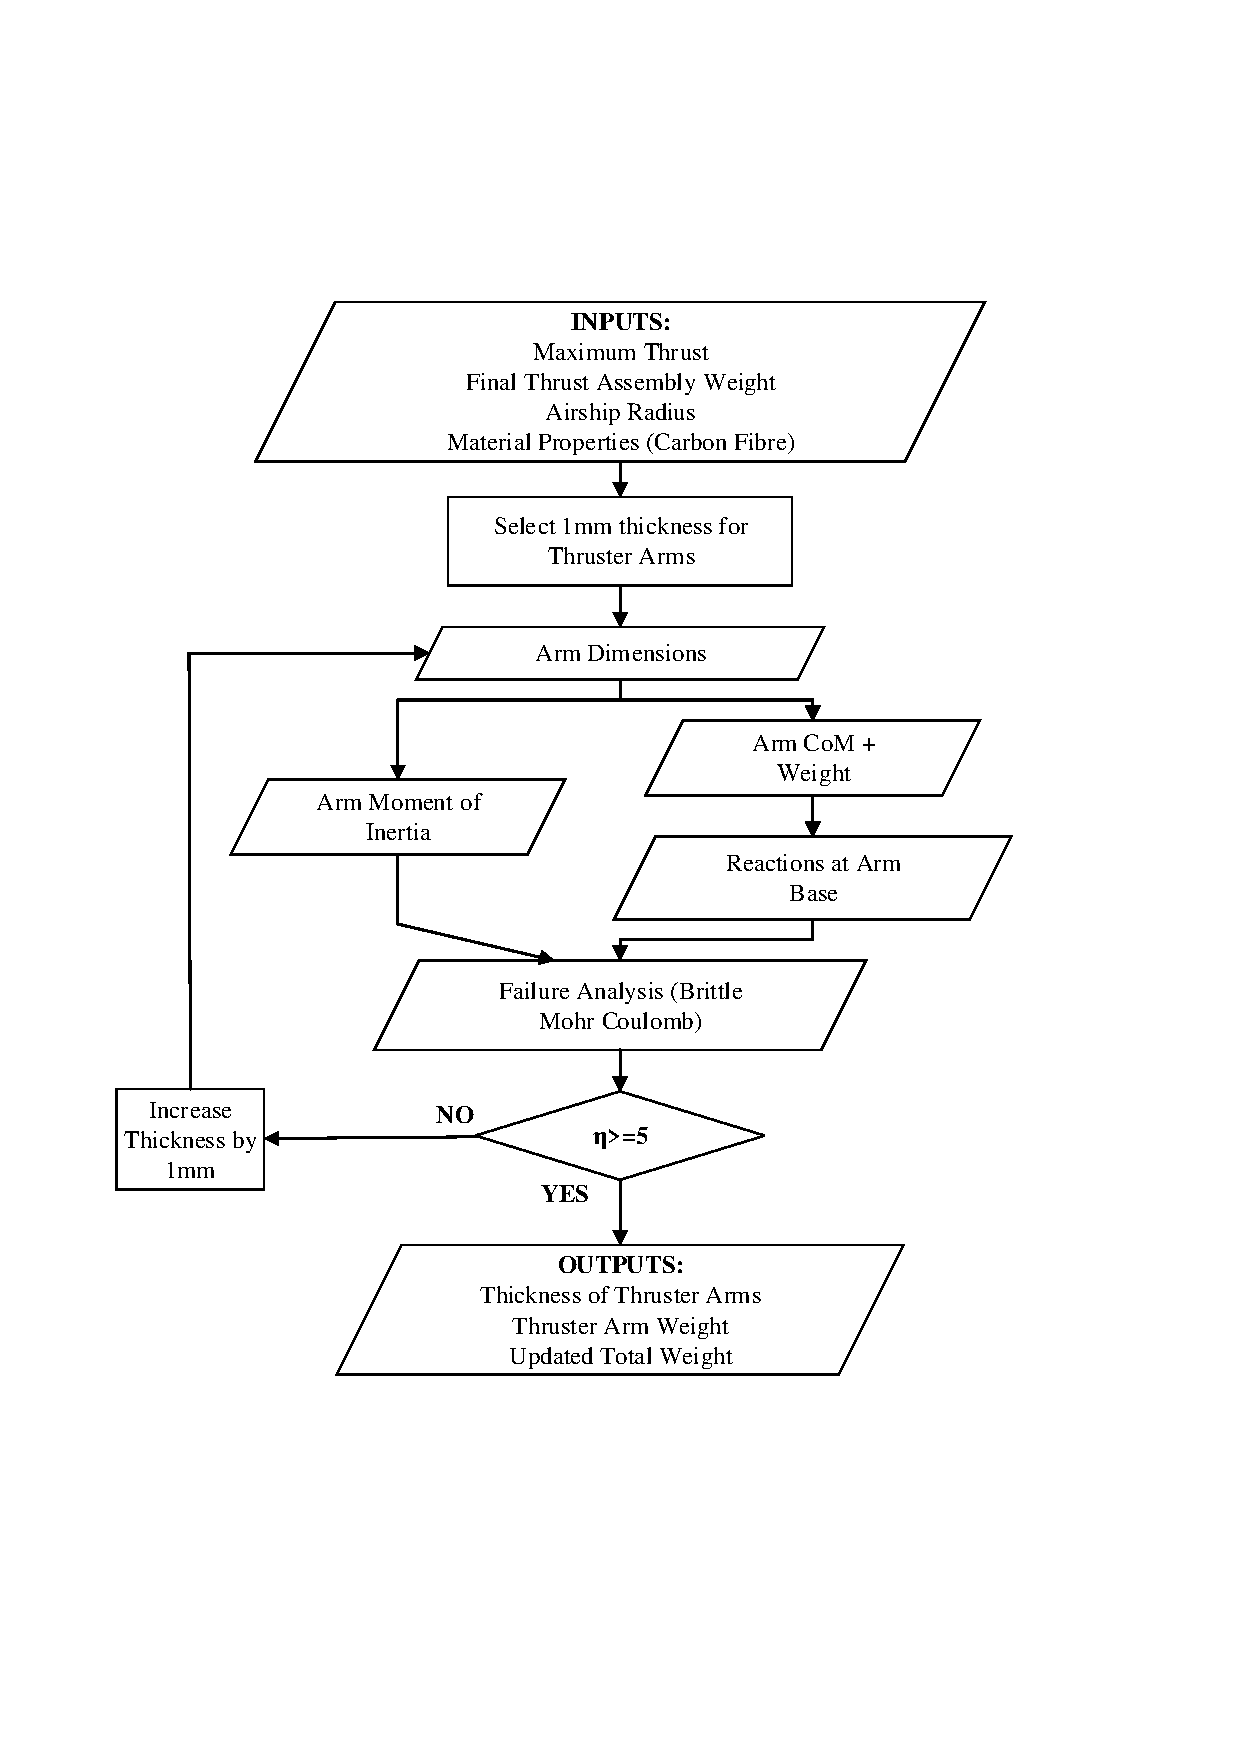
\includegraphics[width=.9\linewidth]{img/paramaterization/thrusterArms.pdf}
	\caption{Parametrization Outline for the Thruster Arms}
	\label{fig:thrusterArmsParametrization}
\end{figure}

The thruster arm analysis is preformed to determine the required arm thickness to meet the specified safety factor. The analysis will also out put the weight of the arms and re compute the weight of the entire thruster assembly and its center of gravity data. In order to run the analysis several inputs are required including the maximum thrust force, thruster assembly weight, the airship radius, and the material properties of the carbon fiber the arms will be fabricated from. In order to minimizing stress concentrations and increase ease of manufacturing the width of the arms is held constant and 30[mm]. This width enables the arms to remain the same width as the section where the keel connector is inserted as seen in FIG???. \\

The scenario for the analysis is that descried in Loading Scenario, Section \ref{loadingScenarios}, Maximum Downward Force show in FIG??? where all forces are with reference to the coordinate system $XYZ$ defined by the pitch of the airship. The analysis begins by computing the reaction forces and moments at the point at the center of the inner radius pf the arms as seen in FIG???. In order to do so the code REF??? sums all the weights of all the thruster assembly components and has them acting at their center of gravity. The following equation \ref{eqn:armCg} is used to solve for the center based on the inner and outer radii $r_o$ and $r_i$. Because of symmetry the center of gravity in Z is the same of that in Y but negative. 
\begin{equation} \label{eqn:armCg}
C.G_{arm} =\frac{4(r_o^3 - r_i^3)}{3\pi(r_o^2 - r_i^2)}
\end{equation}
It also considers the maximum thrust force. once the code solves the reaction forces it computes all considerable stresses acting on the center of the inner radius surface shown in FIG ??. Planar stress in Y is calculated using the equation \ref{eqn:armystress} shown below. The stress is a result of the bending moment about Z
\begin{equation}
\label{eqn:armystress}
\sigma_{y}= \frac{M_{x}c_z}{A r_i (\bar{r} - r)}
\end{equation}
Where $A$ is the area, width $w$ times height $h$, $\bar{r}$ is the center radius of the arm and $r$ is the neutral axis calculated by equations \ref{eqn:armNeutralAxis} shown below. $c_z$ is the distance to the neutral axis $r - r_i$.
\begin{equation} \label{eqn:armNeutralAxis}
\bar{r} = r_i + \frac{h}{2} \hspace{20mm}  r = \frac{h}{ln(r_o/r_i)}
\end{equation}

In addition to the planar stress in Y there is also torsional shear in the XZ plane. This is describes by equation \ref{eqn:torsionShear} from {(Shigley's Machine Design \cite[102]{shigley})}.
\begin{equation} \label{eqn:torsionShear}
\tau_{XZ} = \dfrac{M_{y}}{wh^2}(3+\frac{1.8h}{w})
\end{equation}

The equation accounts for the maximum shear stress in a rectangular cross section which occurs in the center of the wider side which in this case is the width. \\ 

Next the analysis takes both the planar and shear stresses and converted to principle stresses (as shown in Appendix \ref{appendix:cauchy}). These principle stresses are then used to determine the safety factor by Brittle Mohr-Coulomb Theory \cite[227]{shigley}.

\begin{equation}
\eta = \dfrac{S_{ut}}{\sigma _a} \Rightarrow 5 \geq \dfrac{S_{ut}}{\sigma _a}
\end{equation}

A safety factor of five was chosen because there is a relatively high failure likelihood and a failure of this component would result in catastrophic failure of the airship.
\end{document}